\input{./head/uvigo_msthesis.tex}

\usepackage{appendix}
\renewcommand{\appendixname}{Anexos}
\renewcommand{\appendixtocname}{Anexos}
\renewcommand{\appendixpagename}{Anexos}

\usepackage{pdfpages}
\usepackage{graphicx}
\usepackage{grffile}
\usepackage[left=2cm,right=2cm,top=2cm,bottom=2cm]{geometry}

%\hypersetup{pageanchor=false}

\begin{document}
\begin{titlepage}

\Large
\sffamily

\begin{center}
  \begin{tabular}{c}
    \includegraphics[width=0.55\textwidth]{./images/unilogo}
  \end{tabular}
\end{center}

\vfill
\begin{center}
  \huge 
    {\huge Desarrollo de una ensamblador para ARM/THUMB}

\vspace{24pt}
\textcolor{gray}{\small{}}
\end{center}

\vspace*{2cm}
\centerline{{\huge Johan Sebastián Villamarín Caicedo}}

\vfill

\begin{center}
{\large
  Trabajo de Fin de Grado \\
  Escuela de Ingeniería de Telecomunicación \\
  Grado en Ingeniería de Tecnologías de Telecomunicación
}
\end{center}

\vfill
\begin{center}{
{   Tutor \\
    Martín Llamas Nistal
}
}
\end{center}
\vfill
\centerline{\fontsize{11}{13.8} \selectfont Curso 2021/2022}
\end{titlepage}

\newpage
\tableofcontents
\listoffigures
\setcounter{page}{1}


\newpage
\section{Introducción}
{
    % Hoy en día la programación es cada vez una competencia más demandada, con la automatización de tareas siempre surge la necesidad de un software ya sea específico o no. \\
    El desarrollo a bajo nivel de software para una arquitectura específica es siempre de gran complejidad, tanto por el propio lenguaje ensamblador como por la necesidad de disponer del hardware
    específico para probarlo. Debido a esto se recurre a crosscompilers, para compilar código para una arquitectura que no es la del host, y emuladores como QEMU para ejecutar y depurar el programa.
    Existen entornos como \textbf{Xilinx Vitis} que provee de lo necesario para desarrollar y depurar programas integrando QEMU como herramienta de simulación.
    En muchos casos estos entornos resultan pesados de correr y difíciles de configurar. \\

    Para la arquitectura ARM existe \textbf{QtARMSim}, un simulador para ARM programado en python, hace uso de un crosscompiler para compilar el código y después emular la ejecución del mismo.
    Estos entornos tienen en muchos casos dependencias necesarias para su funcionamiento y en el caso de Xilinx Vitis ocupan una gran cantidad de almacenamiento. \\
    % Debido a esto cada vez obtienen mas interés los estudios relacionados con cualquier tipo de desarrollo software (WEB, Android, etc). Entre los distintos lenguajes de programación están los conocidos como \textbf{de bajo nivel o ensamblador}. En estos el programador tiene pleno control sobre los registros de la cpu, habiendo uno específico para cada arquitectura y soportado solo por esta. \\
    
    % Por ello se usa comunmente simuladores para el desarrollo sin necesidad de tener el hardware o incluso en la docencia de este tipo de lenguajes. Permitiendo estos escribir y probar código para una arquitectura que no es la del equipo. Sin embargo, estos simuladores pueden depender de librerías de terceros o programas por lo que su instalación y uso puede no ser siempre tan rápida. Además no todos son intuitivos y/o configurables. \\

    Como solución a esto, y para el caso concreto de ARM Thumb, se decide desarrollar un \textbf{Simulador Web para ARM Thumb}.
    Al tratarse de una plataforma web se simplifica enormemente la instalación dado que bastaría con disponer de cualquier navegador y conexión a internet. Además esto hace que se pueda usar desde cualquier sistema operativo. \\
    
    Actualmente existen distintas alternativas para este propósito como son QtARMSim, ARMThumbSim (web) o OakSim (web).
    Estos entornos ofrecen también la posibilidad de simular código ARM Thumb incluso en el caso de ARMThumbSim un display.
    Estas plataformas sin embargo no permiten la modificación de los valores de la cpu como si hace QtARMSim. Así este proyecto busca integrar ambas partes, la facilidad de uso e interfaz de usuario de una plataforma web, con
    el potencial de modificar aspectos de la cpu como permite QtARMSim. 

    Las tecnologías empleadas para esta plataforma son:
    \begin{enumerate}
        \item \textbf{React}: JavaScript Framework
        \item \textbf{NodeJS}: JavaScript Engine
        \item \textbf{TypeScript}: React - TypeScript
        \item \textbf{React-Redux}: States
        \item \textbf{Docker}: Contenedores
        \item \textbf{Git}: Controlador de versiones
    \end{enumerate}

    \subsection{Arquitectura}
    Los procesadores ARM, a excepción  de los basados en ARMv6-M y ARMv7-M, tienen un total de 37 registros, en algunos casos pueden tener 3 adicionales para distintos usos.
    Un total de 31 registros de 32 bits para uso general y 6 registros de estado. Estos registros no están siempre accesibles al mismo tiempo, dependiendo del modo de ejecución del procesador están disponibles unos u otros.
    Los distintos modos de ejecución son usuario y sistema, FIQ (Fast Interrupt), supervisor, abort, IRQ (Interrupt) y undefined.
    El modo sistema es un modo usuario privilegiado para los sistemas operativos.
    En todos los modos hay disponibles 16 registros de uso general, uno de estado para los flags de la CPU (CPSR) y dependiendo del modo otro más de estado SPSR (Saved Program Status Register), accesible en todos los modos menos en usuario y sistema. \\
    \clearpage
    En este proyecto se considera que la ejecución será siempre en modo usuario por lo que tenemos 16 registros de uso general y un registro de estado CPSR.
    Estos procesadores tienen dos modos de operación, ARM (32-bits word-aligned instructions) y Thumb (16-bit halfword-aligned instructions) que será el modo a emular.
    Como indica la documentación oficial de ARM  en modo Thumb están disponibles los registros inferiores (del 0 al 7) y los registros SP (Stack Pointer o r13), LR (Long Return o r14), PC (Program Counter o r15) y CPSR (sin acceso directo).
    El lenguaje ensamblador tiene acceso limitado a los registros superiores (del 8 al 15) para ser utilizados como un medio temporal de almacenamiento.

    El registro CPSR contiene los flags de condiciones, por ejemplo si después de una suma hubiese overflow el bit C de acarreo (bit 29) se pondría a 1 así como el modo actual de ejecución.
    De los 32 bits de estado los 4 más significativos son los bits N (negativo), Z (cero flag), C (acarreo flag), V (signed overflow). Estos 4 bits son los empleados a la hora de hacer saltos condicionales, es decir para
    continuar la ejecución del programa en otro punto dependiendo de si se cumple o no una condición (por ejemplo si una resta da 0). 
    Dado que el modo de ejecución será siempre Thumb se podrán ignorar los demás bits a la hora de emular la CPU. \\

    Tanto en modo ARM como Thumb soporta los siguientes tipos de datos:
    \begin{enumerate}
        \item \textbf{Palabras}: Valor de 32-bits. Tiene que estar alineado a 4 en la memoria.
        \item \textbf{Medias palabras}: Valor de 16-bits. Alineado a 2.
        \item \textbf{Bytes}: Valor de 8 bits.
    \end{enumerate}
}

\section{Objetivos y metodología de trabajo}
{
    El objetivo principal de este trabajo es desarrollar una plataforma web de software libre, inspirada en \href{https://creatorsim.github.io/creator/}{CREATOR} , que emule la arquitectura ARM Thumb. En la que los usuarios puedan escribir en ensamblador, compilar y probar el programa de forma interactiva.
    Pudiendo ver en todo momento el estado de la cpu, sus registros y flags de estado, así como la memoria y su contenido. \\

    Interpretar el código ensamblador en caso de que no contenga errores, de haberlos se le mostrará al usuario un mensaje de error así como la línea en la que se ha encontrado. 
    
    Funcionalidades mínimas del sistema:
    \begin{enumerate}
        \item \textbf{Comprobación de errores}
        \item \textbf{Simulación del programa}
        \item \textbf{Editor de código}: Editor de texto con syntax highlighting para ARM Thumb.
        \item \textbf{Visualizador de registros}: Panel con los registros de la cpu y su valor. Así como el estado de los flags.
        \item \textbf{Visualizador de programa}: Lista de instrucciones ensamblador que el usuario ha cargado a la cpu.
        \item \textbf{Visualizador de memoria}: Panel con la memoria de la cpu.
    \end{enumerate}

    Como objetivo adicional se busca que la aplicación se lo mas intuitiva posible y permita modificar el estado de la cpu y la memoria que se está simulando. Con facilidades para modificar los valores de ambos. \\
    \clearpage

    A la hora del desarrollo se dividió el proyecto en dos subproyectos, por un lado el emulador y por otro la plataforma web, que integrará siempre la última version del emulador.
    Para ambos subproyectos se emplea un controlador de versiones, en este caso \textbf{git}, con sendos repositorios en github (\href{https://github.com/FreddyJS/armthumb-emul}{ARM Thumb Simulator} y \href{https://github.com/FreddyJS/wthumb}{Web ARM Thumb Simulator}).
    Haciendo uso de \textbf{Github Workflows} para CI/CD, ejecutándose los tests en cada push al repositorio del simulador y para despliegue automático de la web
    gracias a github pages. \\

    La distribución de trabajo fue también en dos fases, la fase inicial se centró en el desarrollo del emulador y crear un entorno de trabajo con tests unitarios.
    Para crear el entorno de trabajo se utilizó \textbf{yarn} como gestor de paquetes y el paquete \textbf{jest} para crear una test suite para el emulador.
    También se creó una interfaz web mínima que integrase el emulador.

    La segunda fase se centró en correción de errores, tests e integración de la plataforma web con el emulador. 
    Por último se abordó el apartado visual empleando \textbf{react bootstrap}.
}

\section{Resultados}
    Se llega a una plataforma web que permite escribir código en ensamblador, parsea y comprueba errores y en caso de que no hubiese simula la ejecución del programa.
    Muestra al usuario los registros y su contenido, los flags de estado, la memoria disponible y el programa cargado.
    Soporta la edición de registros y memoria, se puede introducir un valor específico para cambiar el contenido de estos.

    \subsection{Simulador ARM Thumb}
    {
        Módulo en TypeScript con todas las funciones necesarias para la simulación de código escrito en ARM Thumb.
        Este módulo se desarrolló de forma separada para su posterior integración en el sistema final.
        Gracias a esta división se realizaron pruebas unitarias de cada instrucción implementada
        para asegurar que el comportamiento del simulador es el esperado. \\

        Puede ser empleado por cualquier otra aplicación que use TypeScript. Está dividido en tres grandes partes:
        \begin{enumerate}
            \item \textbf{Compilador}: Comprobación de errores.
            \item \textbf{CPU}: Contiene los registros, flags y la memoria.
            \item \textbf{Tests Unitarios}: Conjunto de tests para cada operación de la cpu.
        \end{enumerate}
    
        % \begin{figure}[h]
        %  \centering
        %     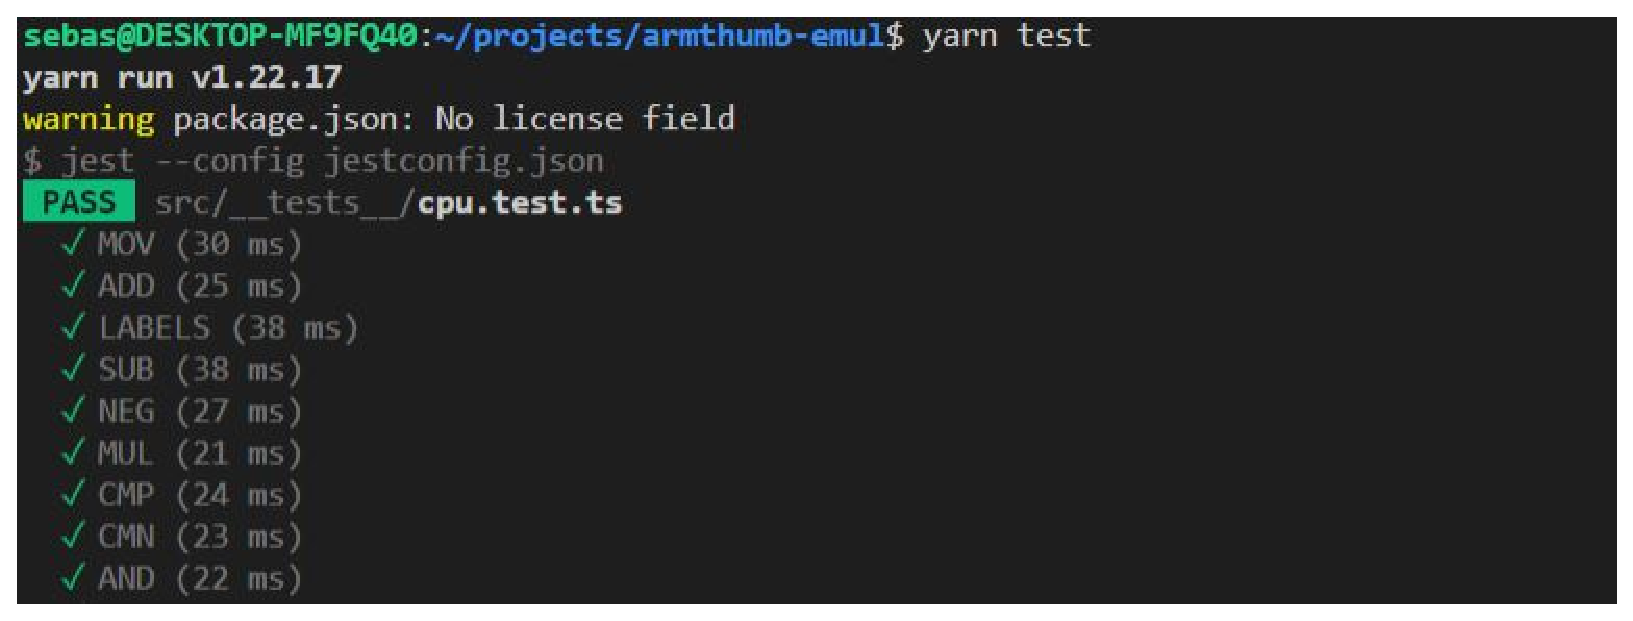
\includegraphics[width=0.85\textwidth]{images/tests}
        %     \caption{Running Test Suite}
        % \end{figure}
        
        % \begin{figure}[h]
        %  \centering
        %     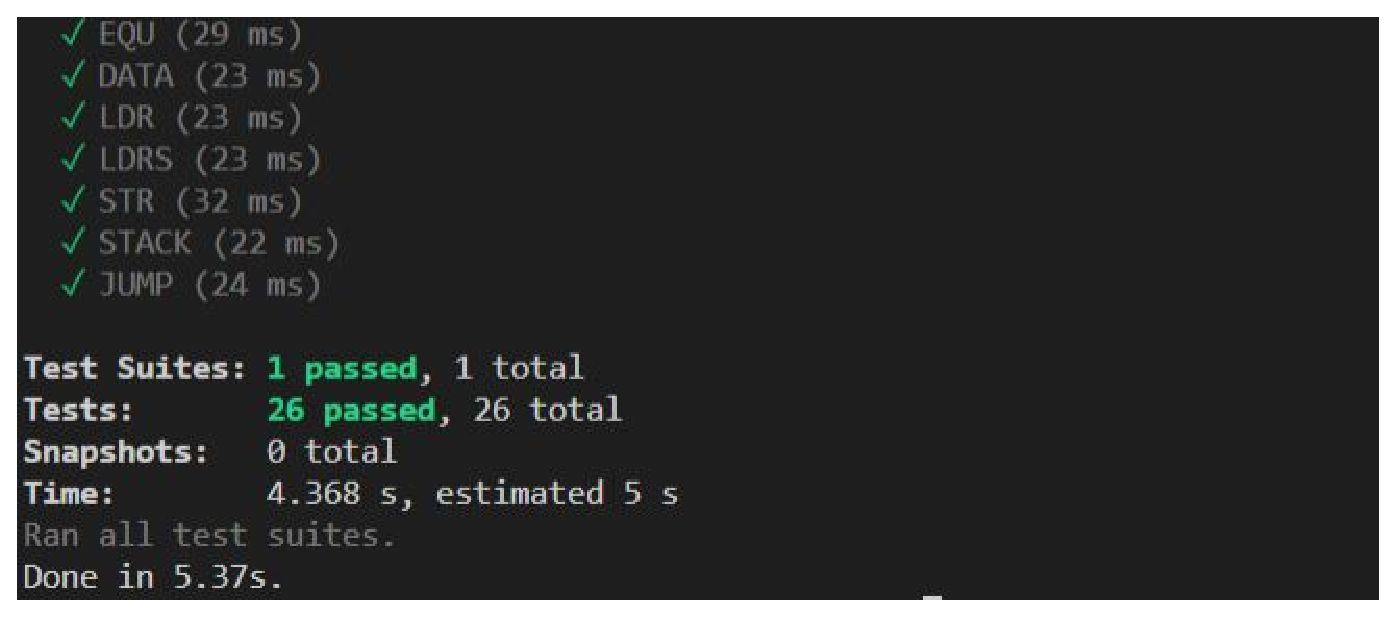
\includegraphics[width=0.85\textwidth]{images/tests2}
        %     \caption{Finished Test Suite}
        % \end{figure}
        \subsubsection{Compilador}
        Implementa la lógica necesaria para la comprobación de errores, interpretar las directivas de ensamblador
        y crear para cada operación un objeto con la información necesaria para su ejecución.
        Gracias a TypeScript se definen los siguientes tipos:
        \begin{enumerate}
            \item \textbf{CompilerError}. Contiene la causa del error y la línea.
            \item \textbf{Operand}. Argumento de una operación, consta de tipo (LowRegister, DecInmediate, ...) y valor.
            \item \textbf{Instruction}. Operación a ejecutar. Campos: operation, operands, break y label.
            \item \textbf{Program}. Programa compilado. Consta de un array de instrucciones y un posible error.
        \end{enumerate}

        Los datos iniciales del programa especificados mediante las directivas de ensamblador (.byte, .asciz, ...)
        son almcenados en un array de números enteros para después cargarse en la cpu junto con el programa.

        Se exporta una única función \textbf{compileAssembly} que recibe una string con el código ensamblador y retorna un objeto
        correspondiente al programa compilado y la memoria inicial que este necesita, el programa podrá tener un error
        para su gestión posterior. Consultar anexo para ver la lista de operaciones y directivas. 

        \subsubsection{ARM CPU}
        Para simular la cpu se define un objeto javascript con los siguientes campos: \\

        \textbf{Registros (regs)} \\
        Objeto javascript script que contiene un par clave valor por cada registro.
        Para ARM Thumb desde r0 a r15 inicializados a 0, menos el registro SP (r13)
        que se inicializa con la dirección de memoria del stack y se actualiza al realizar operaciones en él. \\

        \textbf{CPSR (Z, N, C, V)} \\
        Por simplicidad, y dado que se asume que la ejecución es siempre en el mismo, como se indica previamente,
        se simulan únicamente los 4 bits más significativos (Z, N, C y V), cada uno es miembro del objeto cpu
        de tipo boolean. \\

        \textbf{Memoria (memory)} \\
        Simulada mediante un array de número enteros, tipo number. Dado que javascript emplea 32 bits para representar número enteros
        se inicializa un array de un tamaño por defecto (128), la mitad del array como memoria para almacenamiento y la otra mitad para el stack.
        El tamaño de esta memoria es modificable a la hora de inicializar la CPU. \\
        
        \textbf{Programa (program)} \\
        Se define un tipo de TypeScript \textbf{Instruction}, este objeto tiene el tipo de operación a ejecutar
        (MOV, ADD, SUB, etc), los argumentos de la operación y una posible label. El programa cargado en la CPU se define como un array de estas instrucciones. \\

        \textbf{Error del compilador (error)} \\
        Se define el tipo \textbf{CompilerError} que contiene la causa del error y la línea en la que se ha encontrado.
        Previamente a cargar el código compilado se comprueba si el compilador se ha detenido debido a un error. \\

        Además de estos campos cuenta con los métodos:
        \begin{enumerate}
            \item \textbf{run()}: Ejecuta el programa cargado. Retorna al finalizar la ejecución o al encontrar un breakpoint.
            \item \textbf{step()}: Ejecuta la siguiente instrucción indicada por el registro PC.
            \item \textbf{execute(ins: Instruction)}: Empleado por los dos anteriores, recibe la instrucción a ejecutar y realiza la operación en cuestión.
                Implementa la lógica de cada operación del subconjunto de operaciones de ARM Thumb.
                Activando o desactivando flags según corresponda y modificando los registros o memoria.
            \item \textbf{loadAssembly(assembly: string)}: Llama a \textbf{compileAssembly} para compilar y posteriormente cargar el código ensamblador, en caso de que no haya errores.
                Inicializa la memoria con los valores de la memoria inicial que devuelve el compilador. En caso de haber algún error lo almacena en el correspondiente campo de la cpu
                y retorna sin cargar el programa ni la memoria.
        \end{enumerate}

        \subsubsection{Tests unitarios}
        Durante todo el desarrollo del simulador se tuvo presente la necesidad de realizar tests
        para comprobar el correcto funcionamiento. Por ello se mantuvo en todo momento un conjunto de tests para cada operación.
        
        Cada test tiene un archivo con el código ensamblador a compilar y ejecutar, como primer paso se compila el código
        mediante un crosscompiler para ARM. De no haber error se compila mediante el simulador, se comprueba que no hayan ocurrido errores y por
        último se ejecuta.

        \begin{figure}[h]
         \centering
            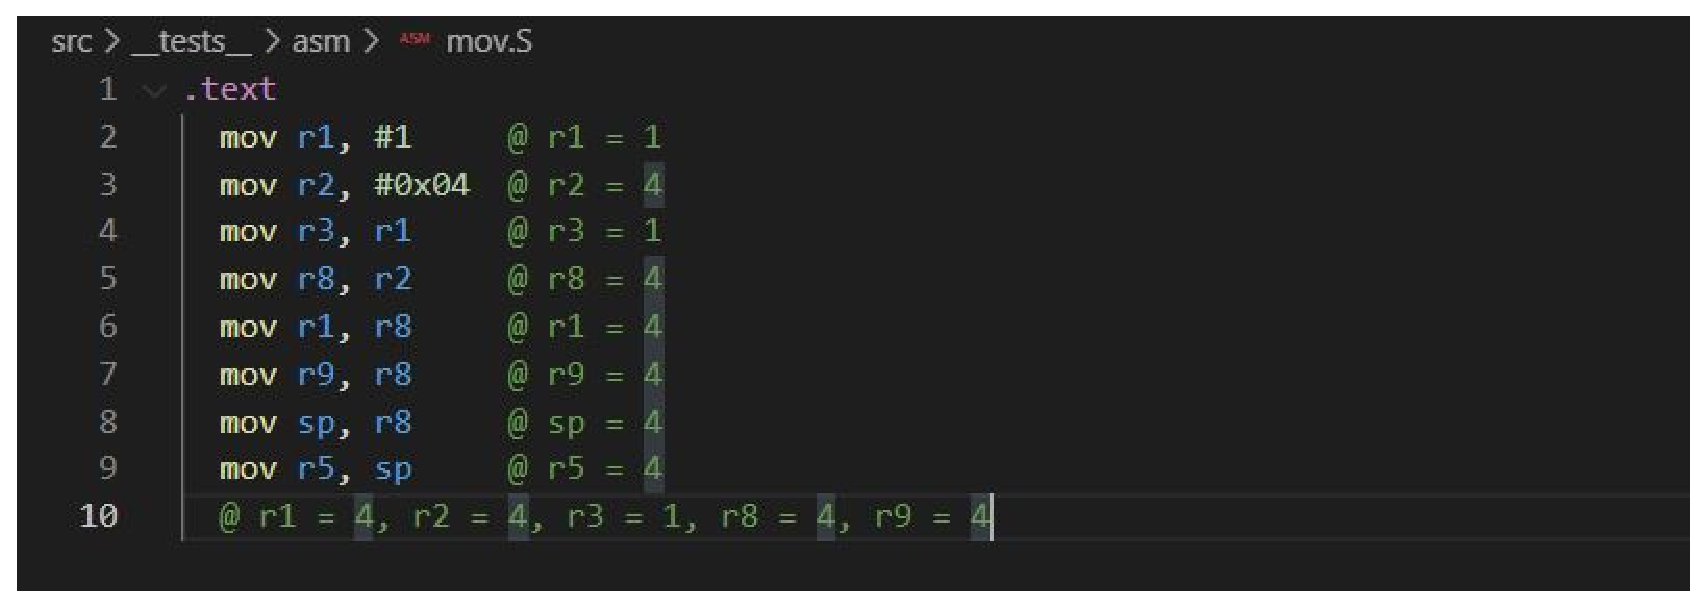
\includegraphics[width=0.85\textwidth]{images/asm}
            \caption{ARM Test Code Example}
        \end{figure}

        \newpage
        Una vez finalizada la ejecución se comprueba si existe el archivo correspondiente con el estado esperado de la cpu.
        De no existir el estado de la cpu tras la ejecución es volcado a un archivo temporal con el nombre del test (add.json.tmp).
        De este modo si el estado es correcto basta con eliminar la extensión .tmp para que en los siguientes tests este sea el estado esperado.
    
        \begin{figure}[h]
         \centering
            \includegraphics[width=0.85\textwidth]{images/state}
            \caption{CPU Expected State Example}
        \end{figure}
        
        Cada test comprueba una instrucción de forma independiente, salvo en algunos casos donde se prueban variantes de una sola en un mismo test (ej: ldr, ldrb, ldrh) u otros
        donde es necesaria otra operación. Por ejemplo para realizar un salto condicional es necesario utilizar una operación previa, por ejemplo de comparación.
        Además de asegurar que el código en ensamblador es correcto mediante el crosscompiler el estado final
        de la cpu se comprobó manualmente mediante el simulador \textbf{QtARMSim}.        
    }
    
    \subsection{Interfaz Web}
    {
        Como interfaz de usuario se desarrolla una plataforma web usando React-TypeScript,
        el objeto cpu se incluye como parte del estado de la cpu gracias a React-Redux lo que
        permite mantener un estado global común para los distintos componentes. El estado global
        de la aplicación consta de tres campos:

        \begin{enumerate}
            \item \textbf{cpu}: El objeto CPU del emulador.
            \item \textbf{assembly}: El código ensamblador que el usuario ha introducido.
            \item \textbf{error}: Mensaje de error para mostrar en la interfaz, es el mismo error de la cpu pero se mantiene en el estado para más rápido acceso, en caso de haber error.
        \end{enumerate}

        Este estado es utilizado por los distintos componentes de la interfaz para mantener siempre la información que se muestra actualizada.
        Cada componente selecciona los campos del estado que necesita acceder y es recargado
        de forma automática si hay algún cambio. \\

        La estética de la interfaz está inspirada en un simulador web que permite simular distintas arquitecturas
        así como crear una propia (\href{https://creatorsim.github.io/creator/}{CREATOR})
        
        \subsubsection{Code Editor}
        {
            Editor de texto con highlighting para ARM Thumb. Hace uso de React CodeMirror que tiene soporte para distintos lenguajes. En este caso se extiende la librería para soportar ARM Thumb. Además incorpora múltiples atajos de teclado para mover, cortar o seleccionar texto.
            
            \begin{figure}[h]
                \centering
                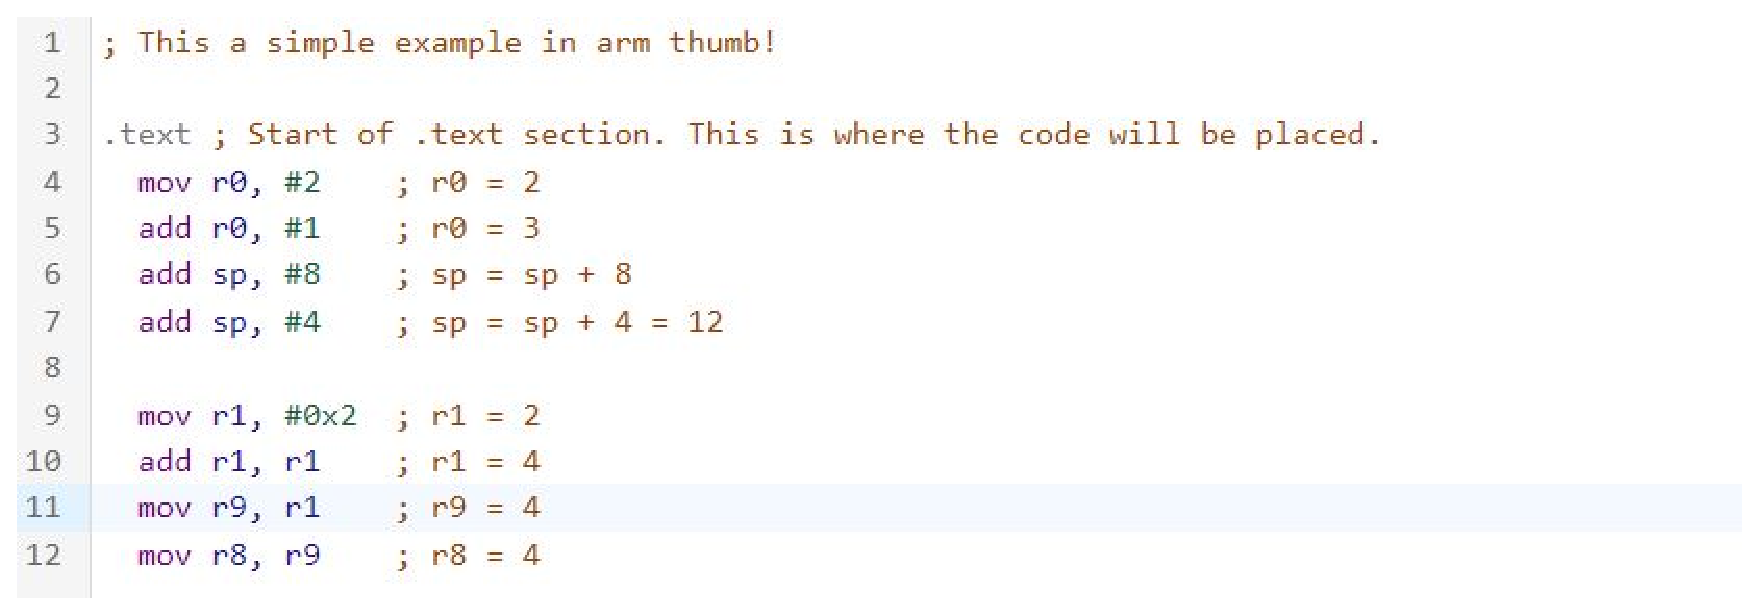
\includegraphics[width=0.85\textwidth]{images/editor}
                \caption{ARM Code Editor}
            \end{figure}

            Este componente muestra en todo momento el valor de \textbf{assembly} del estado de la aplicación y es el encargado de actualizarlo con la entrada del usuario.
            Una vez escrito el programa el usuario puede cargarlo en la CPU mediante el botón de \textbf{Load Program} en la parte superior de la interfaz. \\

            De haber algún error en el código se notificaría al usuario a través de un PopUp indicando la causa y la línea del error.

            \begin{figure}[h]
                \centering
                \includegraphics[width=0.85\textwidth]{images/compilererror}
                \caption{Error Compiling Code}
            \end{figure}
            \clearpage
        }
        
        \subsubsection{Programa}
        {
            Una vez cargado el programa este estará en el panel izquierdo, donde se podrá ver la siguiente instrucción a ejecutar,
            los breakpoints del programa así como todas las demás instrucciones cargadas. \\
            
            \begin{figure}[h]
                \centering
                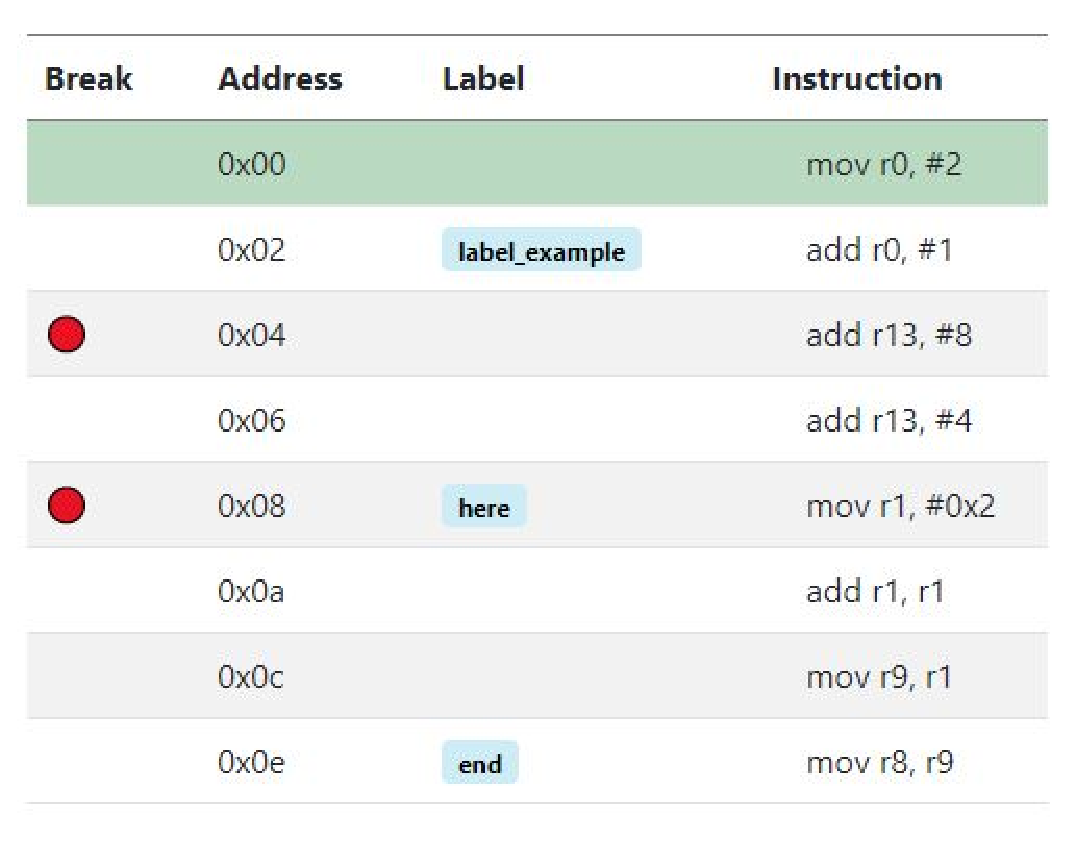
\includegraphics[width=0.8\textwidth, height=0.35\textheight]{images/programa}
                \caption{Loaded Program}
            \end{figure}
            
            Además se pueden poner/quitar breakpoints con un simple click. Para ejecutar el programa una vez cargado tenemos dos opciones:
            \begin{enumerate}
                \item \textbf{Run Code}: Ejecuta el programa hasta que se llega al final o a un breakpoint.
                \item \textbf{Step Into}: Ejecuta instrucción a instrucción el programa.
            \end{enumerate}
        }

        \subsubsection{Registros y flags}
        {
            Este componente se encarga de mostrar en todo momento el valor de cada registro de la cpu.
            En este caso los 16 registros de uso general, además también muestra el estado de los flags.

            Obtiene del estado de la aplicación, gracias a react-redux, el objeto cpu. Este estado se actualiza tras cada operación. De estos 16 registros cabe destacar
            los registros especiales: 

            % En ARM Thumb tenemos acceso a 16 registros, la mitad conocidos como \textbf{Low Registers} y la mitad superior \textbf{High Registers}.
            % Estos registros están siempre representados en pantalla junto con los flags de la cpu. 

            % Los registros inferiores son los del 0 al 7, mientras que los superiores son del 8 al 15.
            % Algunos de los registros superiores son registros con un propósito específico. Estos son:
            \begin{enumerate}
                \item \textbf{R13 (SP)}: Stack Pointer. Se actualiza automáticamente al hacer push o pop
                \item \textbf{R14 (LR)}: Long Return Register. Se actualiza automáticamente al hacer un salto largo.
                \item \textbf{R15 (PC)}: Program Counter Register. Se actualiza automáticamente con la dirección de la próxima instrucción
            \end{enumerate}
            \clearpage

            \begin{figure}[h]
                \centering
                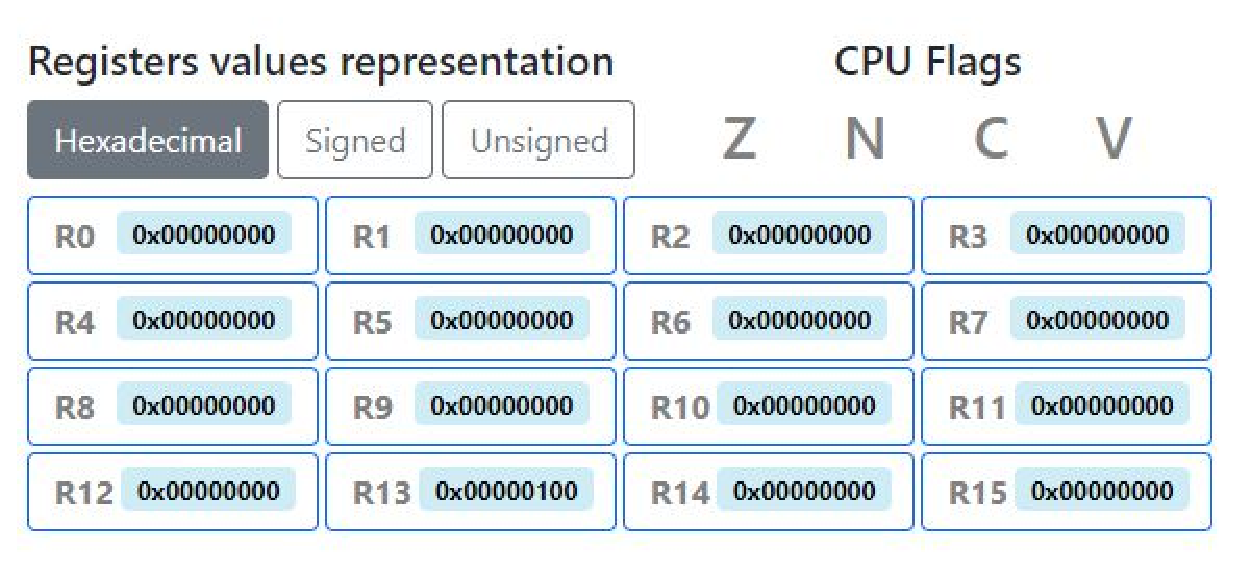
\includegraphics[width=0.85\textwidth]{images/registers}
                \caption{Registers Menu}
            \end{figure}

            Como se puede ver en la figura 6 cada registro aparece por defecto en formato hexadecimal.
            Además se puede cambiar el formato entre hexadecimal, signed y unsigned con un simple click.

            El valor de cada registro puede ser modificado en cualquier momento. Clickando en el registro
            que queremos cambiar abriremos un menú de modificación donde podremos ver el valor actual en
            todos los formatos disponibles así como introducir un nuevo valor.

            \begin{figure}[h]
                \centering
                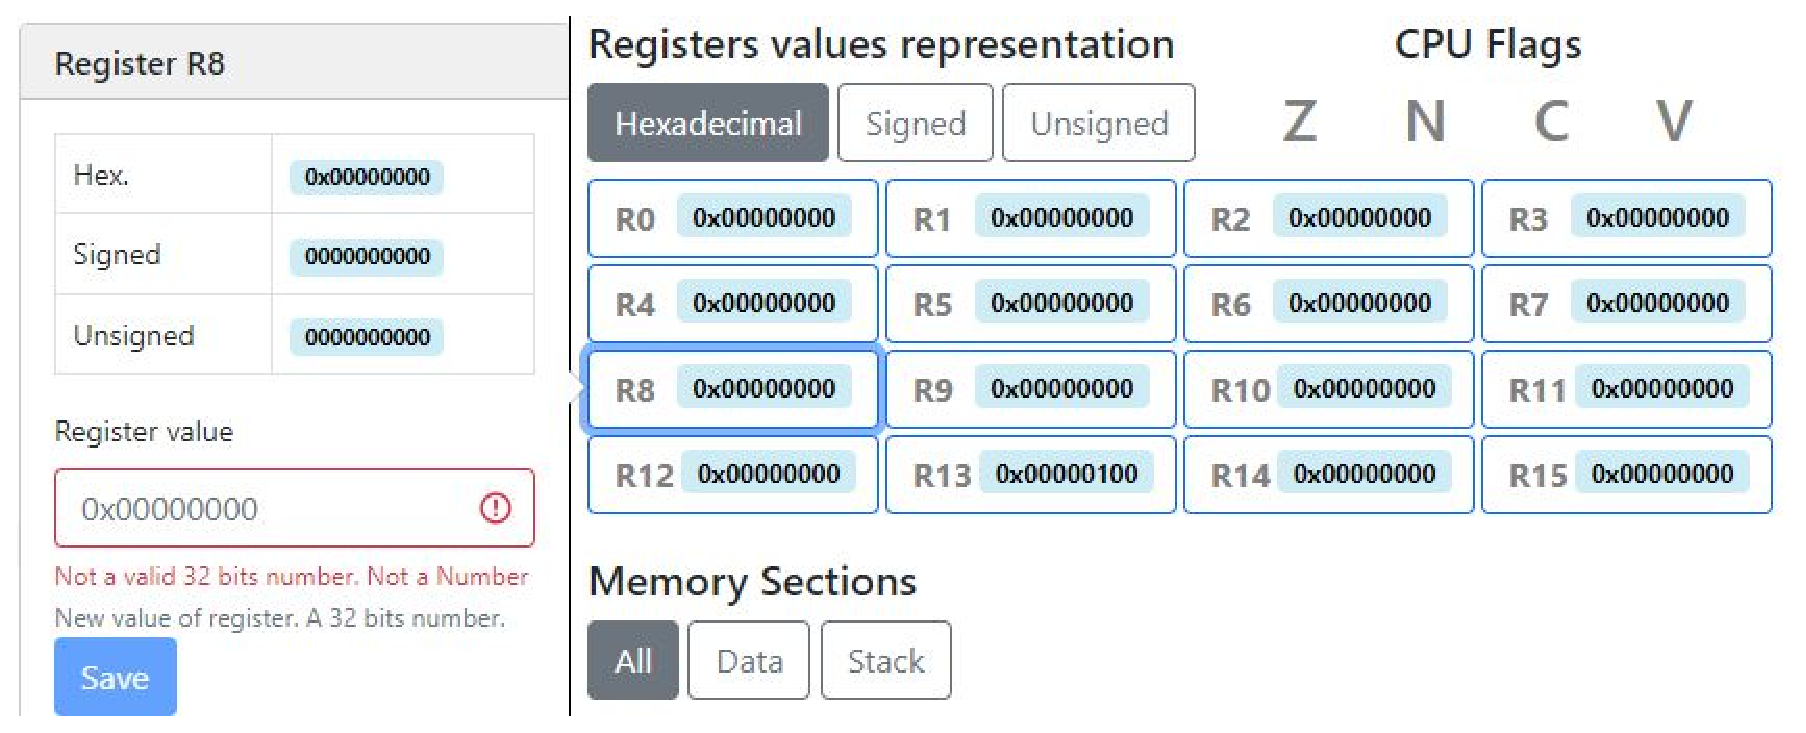
\includegraphics[width=0.85\textwidth]{images/modifyregister}
                \caption{Change Register Value}
            \end{figure}

            Además se comprueba en todo momento que la entrada del usuario sea un nº de 32 bits válido.
            Ya sea en formato hexadecimal o decimal, no se admiten números negativos, y se habilita el botón
            de guardar solo si la entrada es correcta. \\

            En la parte superior derecha tenemos los flags de la cpu. Estos flags se activan en algunas operaciones
            como las de comparar dependiendo del resultado de dicha operación. En caso de ejecutar el programa sin ir
            paso a paso el estado de los flags sería siempre el que hay al final de la ejecución, 
            igual que los registros. Los flags activos se representan en rojo y en gris cuando están a 0.
            \clearpage

            % \begin{figure}[h]
            %     \centering
            %     \includegraphics[width=0.85\textwidth]{images/flags}
            %     \caption{Flags Example}
            % \end{figure}

            % En este ejemplo se compara r0 con un 3. Al ser la comparación una resta y dar esta cero se activa
            % el flag correspondiente Z. Los distintos flags son:
            % \begin{enumerate}
            %     \item \textbf{Z}: Resultado igual a 0
            %     \item \textbf{N}: Resultado negativo
            %     \item \textbf{C}: Bit de acarreo
            %     \item \textbf{V}: Overflow con signo
            % \end{enumerate}
        }

        \newpage
        \subsubsection{Memoria}
        {
            Debajo de los registros está la memoria de la cpu, se inicializa por defecto a 64 palabras (4 bytes)
            como zona libre y 64 más para el stack. Se puede visualizar toda la memoria a la vez, sólo la zona de datos o sólo el stack.

            \begin{figure}[h]
                \centering
                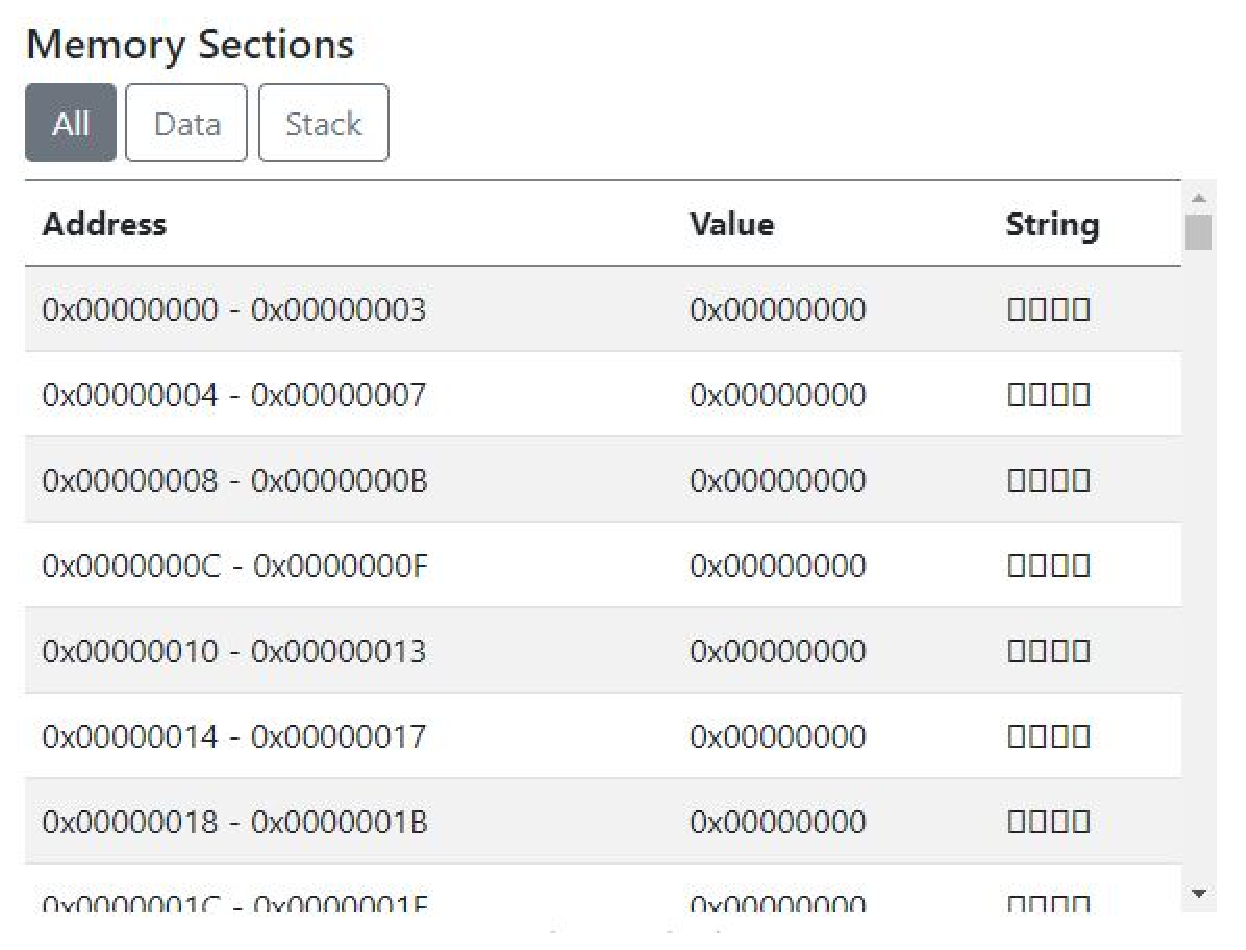
\includegraphics[width=0.85\textwidth]{images/memory}
                \caption{Memory Menu}
            \end{figure}

            El usuario puede utilizar directivas de ensamblador para inicializar la memoria
            con cualquier valor que necesite durante la ejecución. En caso de que el programa necesite más memoria de la disponible esta crece de forma automática, esto puede pasar
            en operaciones como push o en programas que soliciten guardar muchos datos iniciales.

            \begin{figure}[h]
                \centering
                \includegraphics[width=0.85\textwidth]{images/memorydata}
                \caption{Initial Data Example}
            \end{figure}
            Como se puede ver en este ejemplo hay diferentes directivas para almacenar desde strings, bytes, medias palabras
            o palabras. Así como directivas para alinear el próximo dato.

            Además del mismo modo que para los registros los valores de la memoria son fácilmente modificables,
            para ello basta con clickar en la zona de memoria cuyo valor deseamos modificar y se nos abrirá un menú similar al visto
            para modificar un registro. Al igual que para los registros la entrada del usuario se comprueba antes de habilitar el botón de guardar para evitar errores.

            % \begin{figure}[h]
            %     \centering
            %     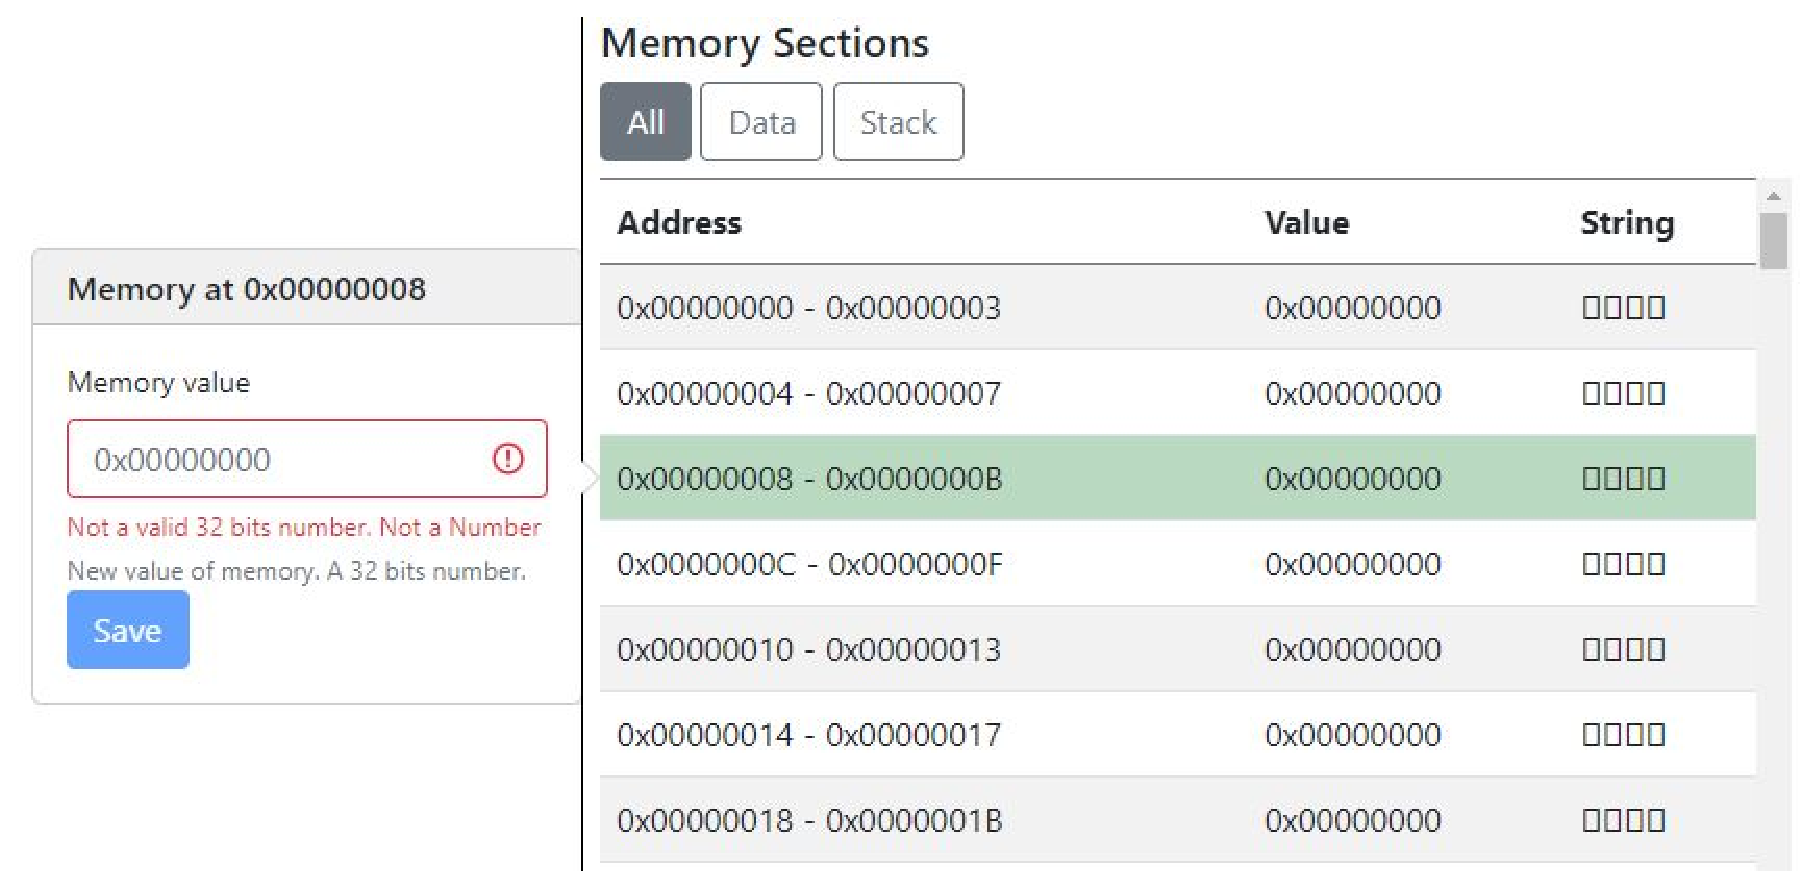
\includegraphics[width=0.85\textwidth]{images/modifymemory}
            %     \caption{Change Memory Value}
            % \end{figure}


            \begin{figure}[h]
                \centering
                \includegraphics[width=0.85\textwidth]{images/stack}
                \caption{Memory Edit Example}
            \end{figure}
        }
    }

\section{Conclusiones y líneas futuras}
{
    Desde el inicio del proyecto se hizo presente la necesidad de implementar pruebas unitarias,
    dada la necesidad de probar cada operación de la cpu. Además de eso la calidad de las pruebas es un factor
    muy importante en todo proyecto ya que de ello depende que se encuentren todos los posibles errores. \\

    Por otra parte el potencial que presenta la disponibilidad de una plataforma web con la capacidad
    de simular código ensamblador de una arquitectura específica es muy elevado, desde para hacer
    pequeñas pruebas de rutinas a por ejemplo el uso desde el hogar sin el equipo del laboratorio. \\

    Una vez finalizado el trabajo se alcanza el objetivo principal, se obtiene una plataforma web
    capaz de interpretar código ensamblador para ARM Thumb. Permitiendo a los usuarios
    programar y simular la ejecución de la cpu. Con comprobación de errores y mensajes de error lo más
    específicos posibles para cada error. Desplegada automáticamente en github pages: \href{https://freddyjs.github.io/wthumb/}{ARM Thumb Emulator}. Además el desarrollo modular permite la integración del simulador
    por parte de cualquier otra aplicación. \\

    Cómo líneas futuras, esta aplicación ganaría aún mas potencial de ser capaz de generar un archivo
    ejecutable para la arquitectura ARM. Mediante el desarrollo de un backend y el uso de un crosscompiler
    se podría enviar el código a compilar y recibir el archivo ejecutable listo para cargar en el equipo donde se
    va a ejecutar. Esto abre además la posibilidad de permitir registrar usuarios, guardar y cargar programas.  
}

\newpage
\section{Referencias}
{
    \begin{enumerate}
        \item \textbf{ARM Developer Documentation}.
            \href{https://developer.arm.com/documentation/ddi0210/c/Programmer-s-Model/Registers/The-Thumb-state-register-set}{https://developer.arm.com/documentation/ddi0210/c/Programmer-s-Model/Registers/The-Thumb-state-register-set}, 
            \href{https://developer.arm.com/documentation/ddi0210/c/Programmer-s-Model/Operating-modes}{https://developer.arm.com/documentation/ddi0210/c/Programmer-s-Model/Operating-modes},
            \href{https://developer.arm.com/documentation/ddi0210/c/Introduction/Instruction-set-summary/Thumb-instruction-summary?lang=en}{https://developer.arm.com/documentation/ddi0210/c/Introduction/Instruction-set-summary/Thumb-instruction-summary?lang=en}
        \item \textbf{CREATOR}.
            \href{https://creatorsim.github.io/creator/}{https://creatorsim.github.io/creator/},
            \href{https://github.com/dcamarmas/creator}{https://github.com/dcamarmas/creator}
        \item \textbf{QtARMSim}.
            \href{http://lorca.act.uji.es/project/qtarmsim/}{http://lorca.act.uji.es/project/qtarmsim/}
        \item \textbf{OakSim}.
            \href{https://wunkolo.github.io/OakSim/}{https://wunkolo.github.io/OakSim/}
        \item \textbf{React Documentation}.
            \href{https://es.reactjs.org/}{https://es.reactjs.org/}
        \item \textbf{React-Redux}.
            \href{https://react-redux.js.org/}{https://react-redux.js.org/},
            \href{https://react-redux.js.org/using-react-redux/usage-with-typescript}{https://react-redux.js.org/using-react-redux/usage-with-typescript}
        \item \textbf{React CodeMirror}.
            \href{https://uiwjs.github.io/react-codemirror/}{https://uiwjs.github.io/react-codemirror/}
        \item \textbf{CodeMirror Documentation}.
            \href{https://codemirror.net/docs/}{https://codemirror.net/docs/},
            \href{https://github.com/codemirror/legacy-modes}{https://github.com/codemirror/legacy-modes}
        \item \textbf{React Bootstrap}.
            \href{https://react-bootstrap.github.io/}{https://react-bootstrap.github.io/}
    \end{enumerate}
}

\newpage

\appendix
\addappheadtotoc

\includepdf[pages={1}, offset=0 3.5cm, pagecommand=\appendixpage\section{Subconjunto de intrucciones ARM Thumb}]{ARMThumbSubset.pdf}
\includepdf[pages={2}, offset=0 7cm, pagecommand=\textbf{}]{ARMThumbSubset.pdf}

\end{document}